\subsection{10}
\begin{myfrag}
Was ist die Gibbs-Duhem Relation? Leite sie her! Was besagt die Gibbs-
Duhem Relation für die Freie Enthalpie G und das Grosskanonische
Potential $\Phi$?
\end{myfrag}
Man betrachte ein System mit der Entropie $S(E,V,N)$. In einem Bruchteil $\alpha$ des Systems ist dann die Entropie $S_\alpha=S(\alpha E,\alpha V,\alpha N)$. Da die Entrope eine intensive Größe ist, gilt
\begin{align}
S=\partd{\alpha}(\alpha S)
	&=\partdd{S}{E}\partdd{\alpha E}{\alpha}+\partdd{S}{V}\partdd{\alpha V}{\alpha}+\partdd{S}{N}\partdd{\alpha N}{\alpha}\\
	&=\frac{1}{T}E+\frac{p}{T}V+\frac{\mu}{T}N\\
	&\mathrel{\Rightarrow} E=TS-pV+ \mu N
\end{align}
Dies ist die Gibbs-Duhem-Relation. Für die Gibbs'sche freie Energie bzw. das Großkanonische Potential schreibt damit man $G = E - T S + pV = \mu N$ bzw. $\Phi = E - T S - \mu N = -pV$

\section{Thermodynamische Größen}
\subsection{11}
\begin{myfrag}
Definiere die Wärmekapazitäten $C_p$ und $C_V$, die Kompressibilität $\kappa_T$, den
Ausdehnungskoeffizienten $\alpha$ und den Spannungskoeffizienten $\gamma$ als
partielle Ableitungen. Berechne $\alpha, \gamma$, $C_p$ und $C_V$ für ein ideales
klassisches Gas.
\end{myfrag}
Es gelten die Definitionen
\begin{align}
	C_p&=\left(\frac{\delta Q}{\partial T}\right)_p=T\partddd{S}{T}{p}=\partddd{E}{T}{p},\\
	C_V&=\left(\frac{\delta Q}{\partial T}\right)_V=T\partddd{S}{T}{V}=\partddd{H}{T}{V},\\
	\alpha&=\frac{1}{V}\partddd{V}{T}{p, N}=\partddd{\logn V}{T}{p, N},\\
	\kappa_T&=\frac{1}{V}\partddd{V}{p}{T}=\partddd{\logn V}{p}{T}\text{ und}\\
	\gamma&=\frac{1}{p}\partddd{p}{T}{V}=\partddd{\logn p}{T}{V}.
\end{align}
Im Idealen Gas gelten die Zustandsgleichungen $pV=Nk_BT$, $E=\frac{3}{2}Nk_BT$ und $S=Nk_B\left(\logn V+\frac{3}{2}\logn T+\mathsf{const.}\right)$. Man errechnet damit
\begin{align}
	C_p&=\partddd{E}{T}{p}=\frac{3}{2}Nk_B,\\
	C_V&=\partddd{H}{T}{V}=\partddd{E+pV}{T}{V}=\frac{5}{2}Nk_B,\\
	\alpha&=\partddd{\logn V}{T}{p, N}=\frac{1}{T},\\
	\kappa_T&=\partddd{\logn V}{p}{T}=\frac{1}{p}\text{ und}\\
	\gamma&=\partddd{\logn p}{T}{V}=\frac{1}{T}.
\end{align}

\subsection{12}
\begin{myfrag}
Leite die Umkehrrelation und die zyklische Relation für partielle
Ableitungen her.
\end{myfrag}
\begin{enumerate}[(a)]
\item Die Umkehrrelation ergibt sich direkt aus dem Satz über die Umkehrfuntion, sofern die Funktion $y(x)$ und $x(y)$ sowie ihre Ableitungen existieren.
\item TODO
\end{enumerate}
\subsection{13}
\begin{myfrag}
Zeige dass der Druck und allgemeine generalisierte Kräfte mit Hilfe einer
Ableitung der Entropie berechnet werden können.
\end{myfrag}
Sei die Kraft $f$ zum thermodynamischen Potential $\alpha$ konjugiert. Unter Verwendung der zyklischen Relation gilt
\begin{equation}
	f=\partddd{E}{\alpha}{S}\overset{\text{zykl. Rel.}}=\partddd{E}{S}{\alpha}\partddd{S}{\alpha}{E}=T\partddd{S}{\alpha}{E}
\end{equation}
\subsection{14}
\begin{myfrag}
Leite einen Ausdruck für den Spannungskoeffizienten $\gamma$ als Funktion des
Ausdehnungskoeffizienten $\alpha$ und der Kompressibilität $\kappa_T$ her.
\end{myfrag}
Nach der zyklischen Relation ist
\begin{align}
	\partddd{V}{T}{p}\partddd{T}{p}{V}&=-\partddd{V}{p}{T}\\
	V\alpha\cdot\frac{1}{p\gamma}&=-V\kappa,\\
	\Rightarrow\qquad\qquad\gamma&=-\frac{\alpha}{p\kappa}.
\end{align}
\subsection{15}
\begin{myfrag}
Leite die vier Maxwell Relationen her!
\end{myfrag}
Aus den totalen Differentialen der thermodynamischen Potentiale ergibt sich
\begin{align}
	\dif E = T \dif S - p\dif V &\Rightarrow \partddd{T}{V}{S,N}=-\partddd{p}{S}{V,N},\\
	\dif F = -S \dif T - p\dif V &\Rightarrow \partddd{S}{V}{T,N}=\partddd{p}{T}{V,N},\\
	\dif H = T \dif S - V\dif p &\Rightarrow \partddd{T}{p}{S}=\partddd{V}{S}{p}\text{ und}\\
	\dif E = -S \dif T - V\dif p &\Rightarrow \partddd{S}{p}{T}=-\partddd{V}{T}{p}.
\end{align}
\subsection{16}
\begin{myfrag}
Leite einen allgemeinen Ausdruck von physikalischen Parametern für die
Differenz zwischen den Wärmekapazitäten $C_p$ und $C_V$ her.
\end{myfrag}
Aus $\dif S = \partddd STV\dif T+\partddd SVT\dif V$ folgt durch Ableiten nach T (bei konstantem Druck)
\begin{align}
	\partddd STp &=\partddd STV\partddd TTp+\partddd SVT\partddd VTp\\
	C_p&=C_V+T\partddd SVT\partddd VTp\\
	C_p&=C_V+VT\frac{\alpha^2}{\kappa_T}
\end{align}

\subsection{17}
\begin{myfrag}
Betrachte die Druckabhängigkeit p(V) für einen adiabatischen Prozess. Leite mit
Hilfe geeigneter Relationen einen allgemeinen Ausdruck für $\partddd VpS$ her. Was ist die Adiabatengleichung unter der Annahme, dass $\sigma = \dfrac{C_p\gamma}{C_V\alpha}$ konstant bleibt? Was ist $\sigma = \dfrac{C_p\gamma}{C_V\alpha}$ für ein ideales klassisches Gas?
\end{myfrag}
TODO

\section{Kreisprozesse und Wärmekraftmaschinen}
\subsection{18}
\begin{myfrag}
Was ist mit dem Begriff reversibler Kreisprozess gemeint? Was ist die praktische
Bedeutung?
\end{myfrag}
Ein reversibler Kreisprozess ist ein periodischer Prozess, der nur aus reversiblen Prozessen besteht, die auf die selbe Arbeitssubstanz wirken. Praktische Bedeutung hat der Carnot-Prozess, der den maximal möglichen Wirkungsgrad realisiert. Dies kann mittels des folgenden Gedankenexperiments überprüft werden:
\begin{figure}[H]
\centering
%h\begin{tabular}{cc}
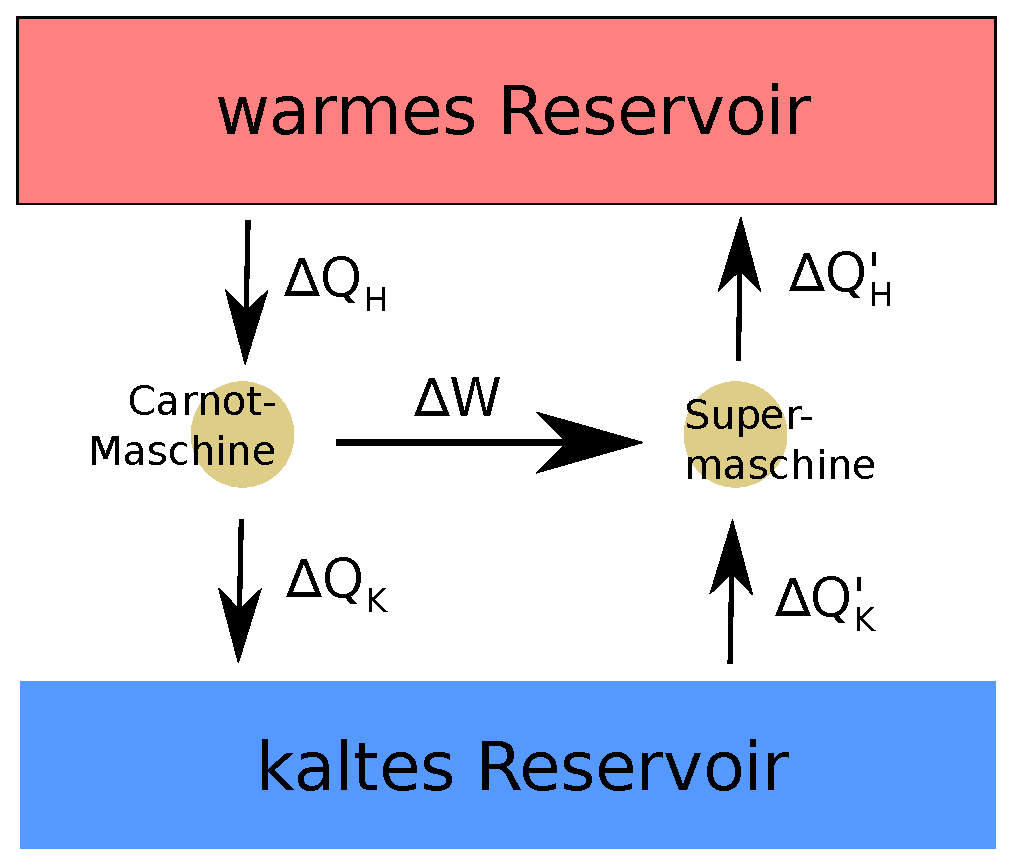
\includegraphics[width=0.45\textwidth]{Bilder/fr18.pdf}%&
\caption{Aufbau zur Bestätingung des maximalen Wirkungsgrades bei der Carnot-Maschine}
%\end{tabular}
\end{figure}
Die Carnotmaschine betreibe mit der frei werdenden Arbeit eine weitere Maschine als Wärmepumpe. Wir nehmen nun an, dass die Super-Maschine einen Wirkungsgrad $\eta>\eta_C$, des Wirkungsgrades der Carnot-Maschine habe. Dann müsste die Supermaschine mehr Wärme ins warme Reservoir transporieren, als die Carnot-Maschine verbraucht. Global heißt das, dass Wärme spontan vom kalten zum warmen Reservoir fließt, was dem zweiten Hauptsatz wiederspricht. Damit haben alle anderen reversiblen Kreisprozesse höchstens einen kleineren Wirkungsgrad. Da man dann das Experiment umdrehen und die Supermaschine zum Treiben des Stirlingmotors nutzen kann, müssen die Wirkungsgrade gleich sin.

\subsection{19}
\begin{myfrag}
Wie sind die Wirkungsgrade für Motoren, Kühlmaschinen und Wärmepumpen
definiert?
\end{myfrag}
Es gilt
\begin{align}
	\eta&=-\frac{\Delta W}{\Delta Q_H}\text{ für Motoren,}\\
	\eta_K&=-\frac{\Delta W}{\Delta Q_K}\text{ für Kältemaschinen,}\\
	\eta_W&=-\frac{\Delta W}{\Delta Q_W}\text{ für Wärmemaschinen.}
\end{align}
